\section{Ignitions}
\pgfdeclareimage[width=1.0\paperwidth]{header-image}{header_images/red_lightn}

\begin{frame}
    \frametitle{Igntions}
    \framesubtitle{Humans and Natural < Humans + Natural}

    \begin{tikzpicture}
        \node[anchor=south west,inner sep=0] (image) at (0,0) {
            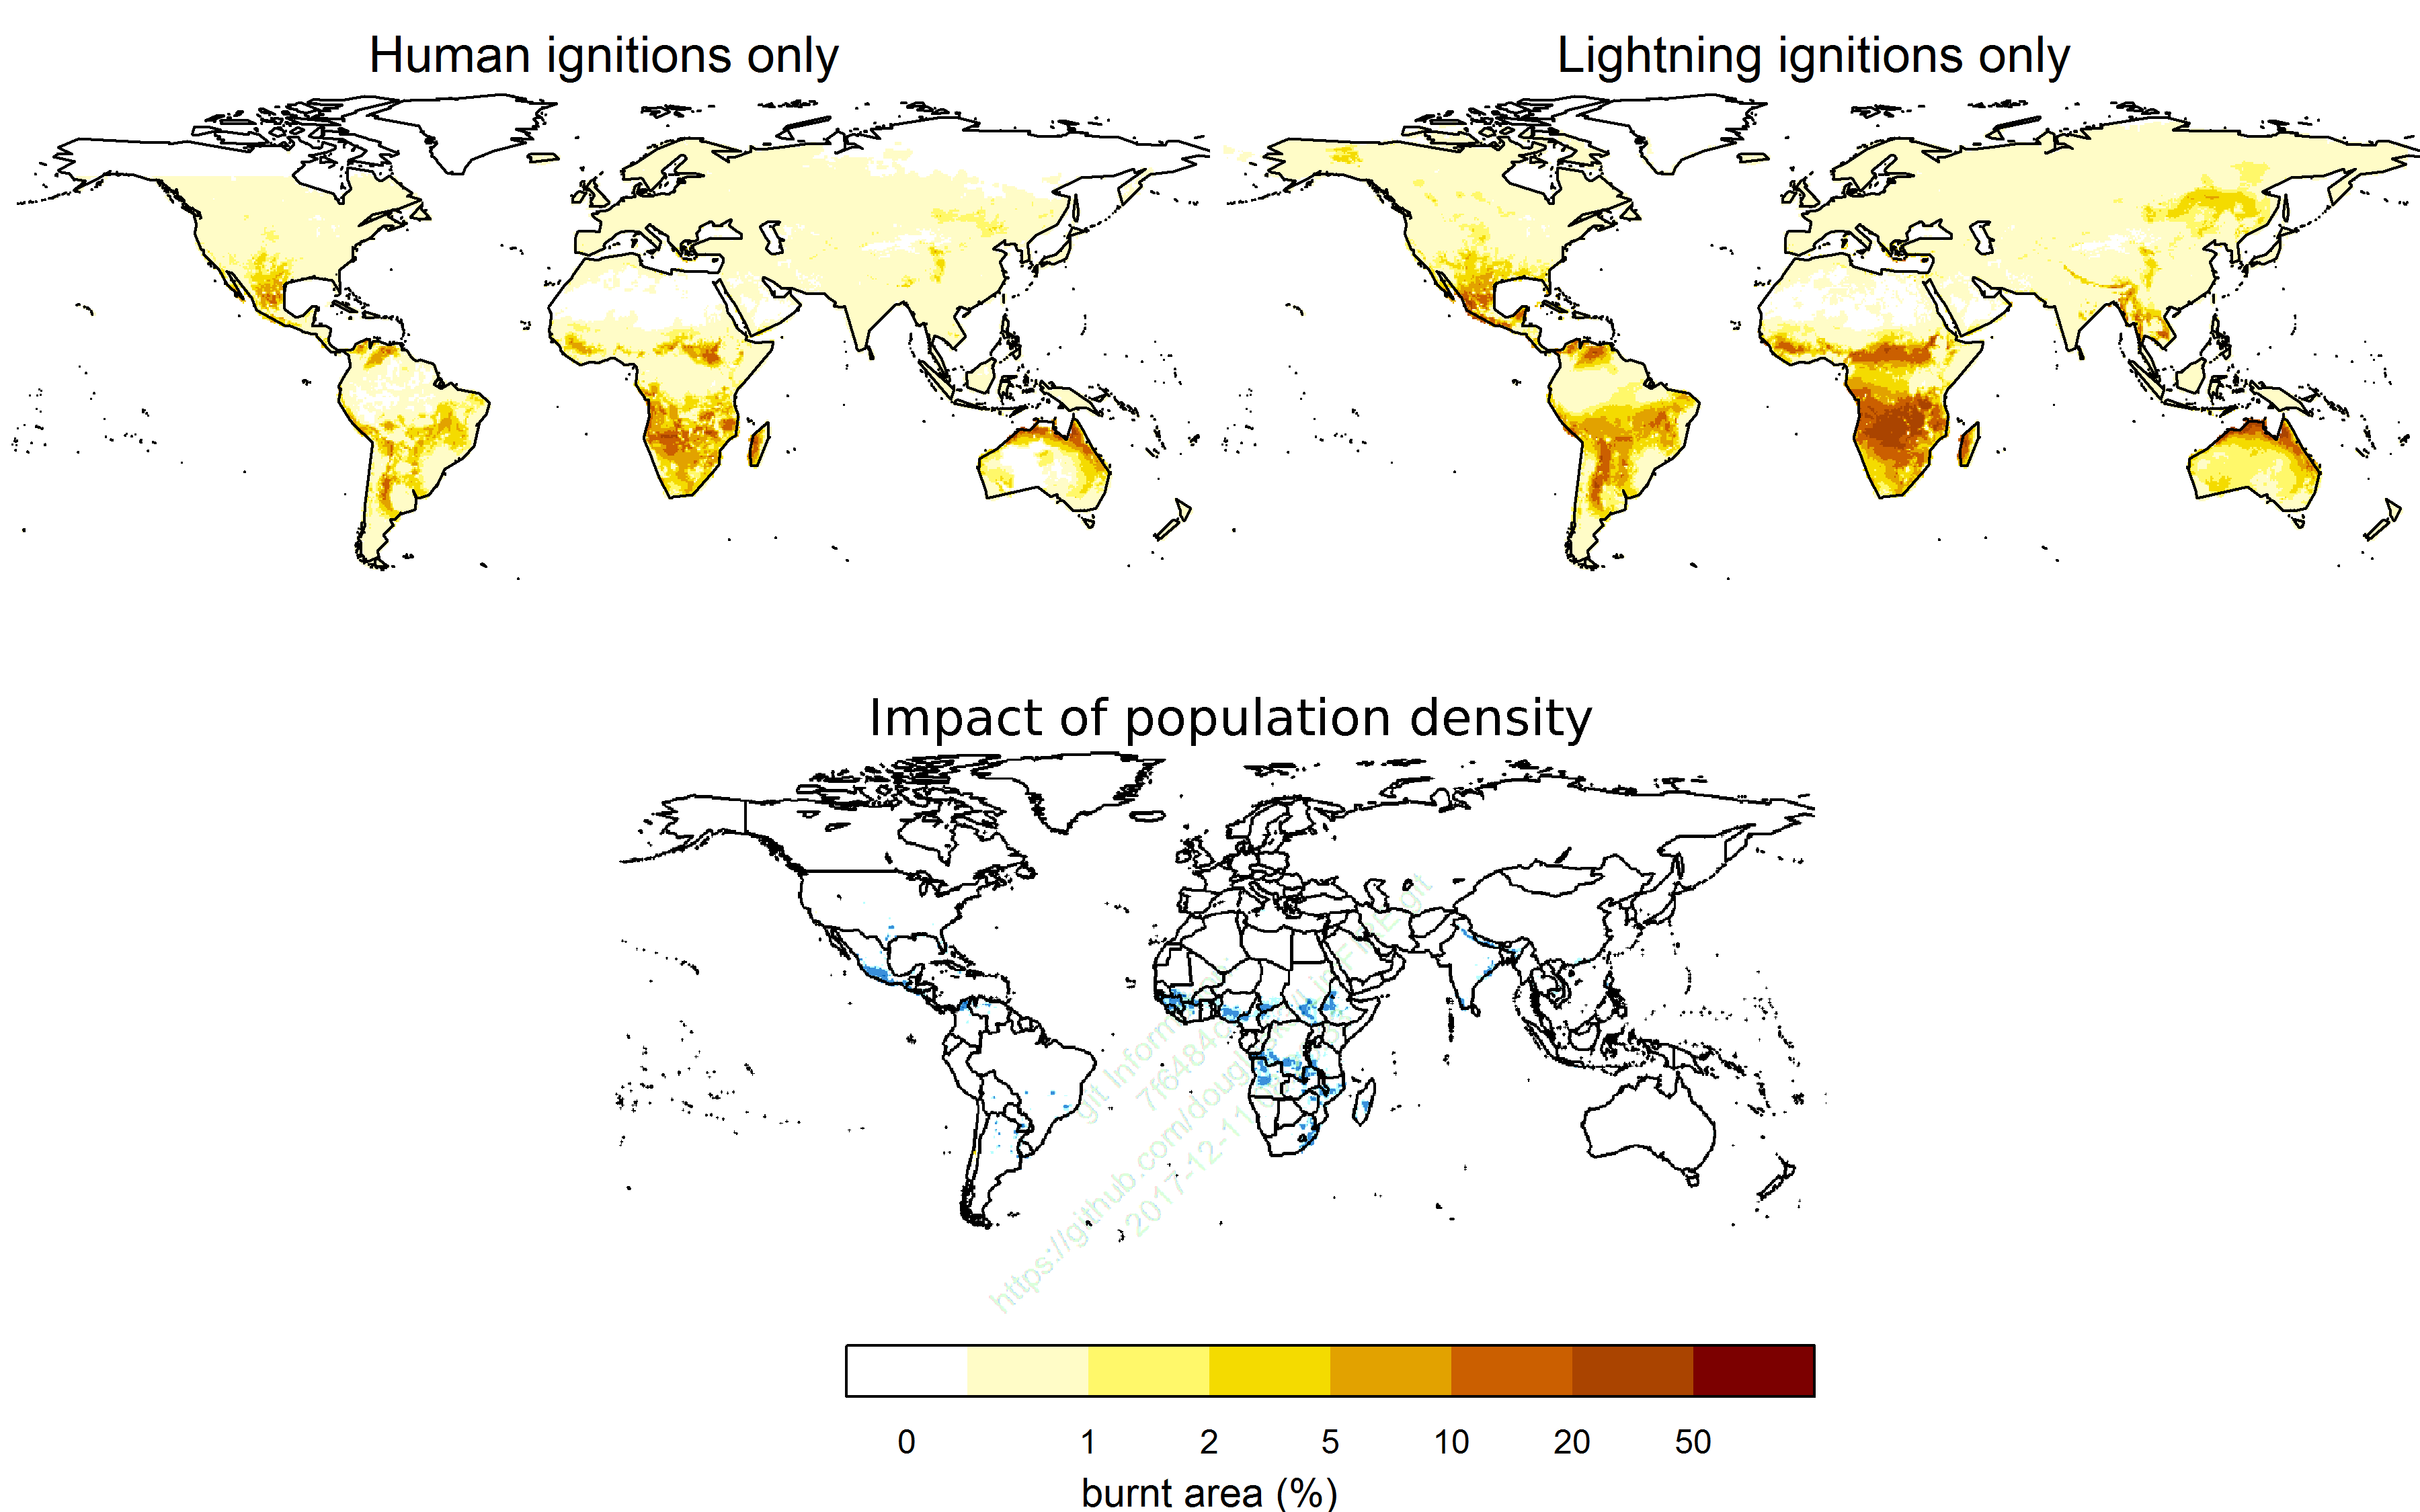
\includegraphics[width=11.0cm]{images/igntitions/IgntionInfoSourceAdding}
        };

        \visible<-1> {\draw[white, fill = white] (5.5,5) -- (12.0,5) -- (12.0,8.4) -- (5.5,8.4) -- (5.5,5);}
        \visible<-2> {\draw[white, fill = white] (0.0,0) -- ( 5.5,0) -- ( 5.5,4.0) -- (0.0,4.0) -- (0.0,0);}
        \visible<-3> {\draw[white, fill = white] (5.5,4) -- (12.0,4) -- (12.0,0.0) -- (5.5,0.0) -- (5.5,4);}
        \visible<-4> {\draw[white, fill = white] (0.0,0) -- (12.0,0) -- (12.0,1.0) -- (0.0,1.0) -- (0.0,0);}
    \end{tikzpicture}

\end{frame}

\begin{frame}
    \frametitle{Igntions}
    \framesubtitle{Which is more important}
    %\node[anchor=south west,inner sep=0] (image) at (0,0) {
    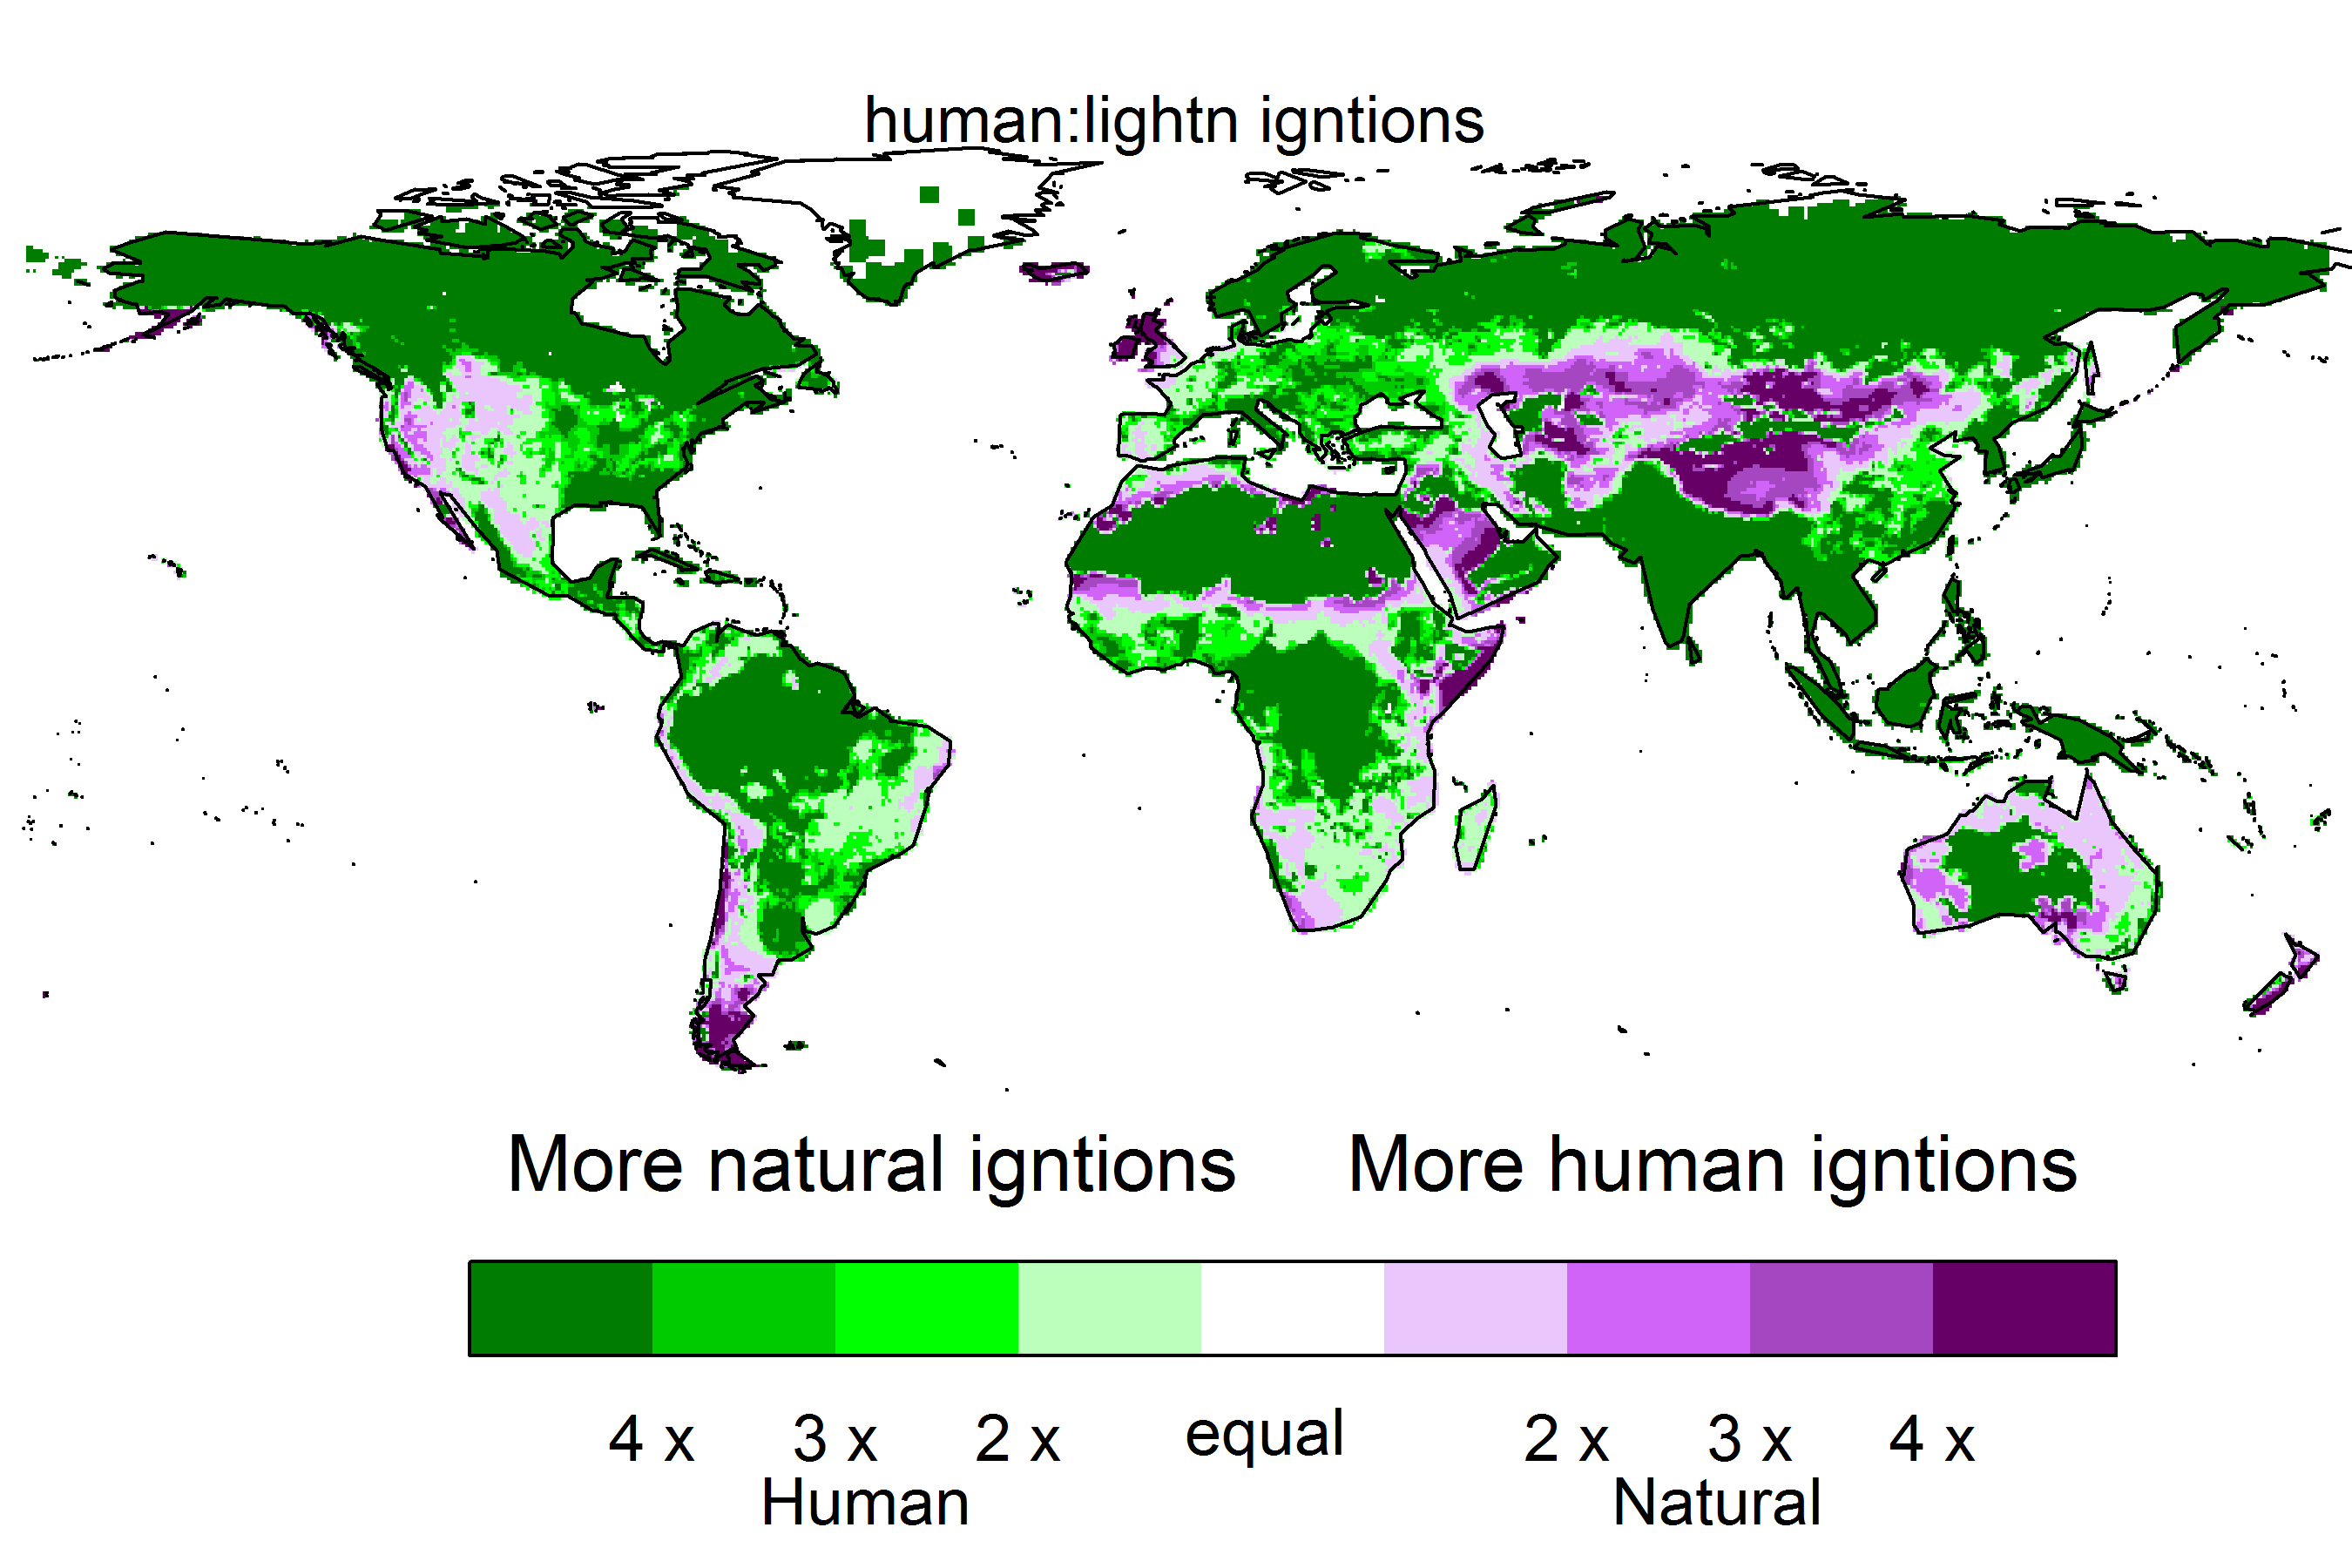
\includegraphics[width=11.0cm]{images/igntitions/IgntionInfosourceImportance}

\end{frame}

%\begin{frame}
%    \frametitle{Igntions}
%    \framesubtitle{Igntion saturattion and manipulation}
%\end{frame}
